\documentclass{article}

\usepackage{nips_2018_author_response}

\usepackage[utf8]{inputenc} % allow utf-8 input
\usepackage[T1]{fontenc}    % use 8-bit T1 fonts
\usepackage{hyperref}       % hyperlinks
\usepackage{url}            % simple URL typesetting
\usepackage{booktabs}       % professional-quality tables
\usepackage{amsfonts}       % blackboard math symbols
\usepackage{nicefrac}       % compact symbols for 1/2, etc.
\usepackage{microtype}      % microtypography
\usepackage{graphicx}
\usepackage{float}
\begin{document}

We first would like to thank all reviewers for taking the time to provide thoughtful comments about our work.


\textbf{Comments for reviewer 1:}

\textit{"I would suggest the author to remove the control part and focus more on the value approximation. (...) To me, the effect of control by the improved value function approximation is indirect."}


We believe the control experiments showcase the potential for temporal regularization to be incorporated in more recent empirical work even though, as pointed out, the effect in the control case is more indirect. However it can be argued that a faster policy evaluation (mixing time) can improve performance in control (Kearns et al., ``Near-optimal reinforcement learning in poloynomial time". Machine Learning. 2002). These experiments support the claim that the proposed approach is really usable in practice, and therefore has potential to have more impact than complex strategies that are hard to extend or scale.  But if all reviewers agree, we could remove this part.


\textit{"The comparison study of different temporal regularization methods is incomplete"}

Though the original experiments were focused on regularization from the past value only (aiming for simplicity), it is possible to consider more complex and powerful regularizers. Let us study a different time series prediction model, namely exponential averaging, where $    \widetilde{v}(s_t) = (1-\lambda)v(s_t) + \lambda \widetilde{v}(s_{t-1})$. The complexity of such models is usually articulated by hyper-parameters, allowing complex models to improve performance by better adapting to problems. However, this potential gain comes at the price of a potential loss in case of model misfit.
We illustrate this by comparing the performance of regularization using the previous state and an exponential averaging of all previous states on the room experiment (Sec. 5.4) and on the noisy walk experiment (Sec. 5.5).
Fig.~\ref{fig:room} shows the average error on the value estimate using past state smoothing, exponential smoothing, and without smoothing. In this setting, exponential smoothing transfers information faster, thus enabling faster convergence to the true value.
However it's important to note that the exponential model involves an extra smoothing hyper-parameter $\lambda$. Fig.~\ref{fig:smoothing} shows the absolute distance from the regularized state estimate (using exponential smoothing) to the optimal value while varying $\lambda$ (higher $\lambda$ = more smoothing). Increasing smoothing improves performance up to some point, but when $\lambda$ is not well fit the bias becomes too strong and performance declines. This is a classic bias-variance tradeoff. These results can be added to the paper.

\begin{figure}[H]
\begin{minipage}[c]{0.48\linewidth}
\centering
\includegraphics[scale=0.45]{fig/room_exp.png}
\caption{Benefits of complex regularizers on the room domain.}
\label{fig:room}
\end{minipage}
\hfill
\begin{minipage}[c]{0.48\linewidth}
\centering
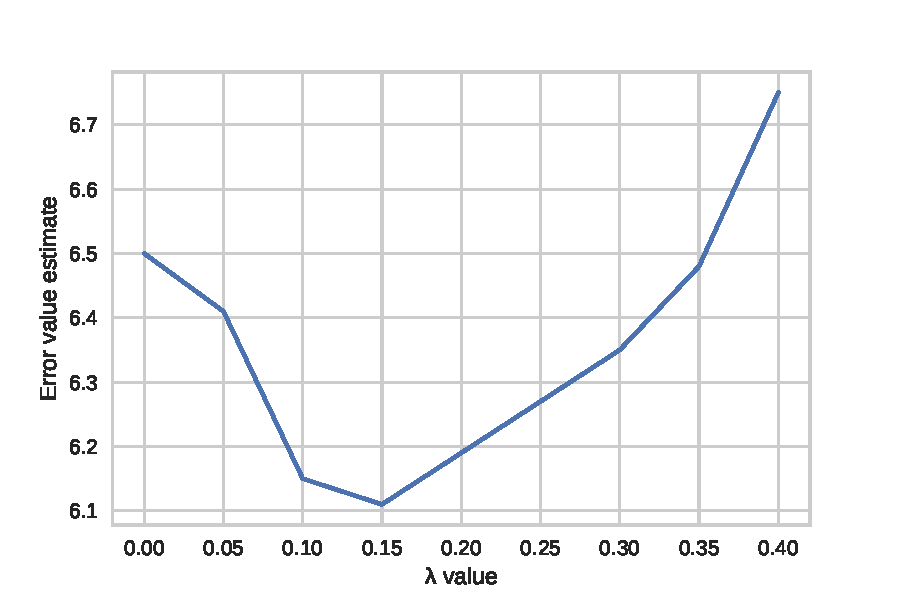
\includegraphics[scale=0.45]{fig/error_noisy.png}
\caption{Impact of complex regularizer parameterization ($\lambda$) on the noisy walk.}
\label{fig:smoothing}
\end{minipage}
\end{figure}


\textbf{Comments for reviewer 2:}

\textit{"(...) more details on how PPO is extended with temporal regularization. Is (10) applied with a finite N?"}

PPO uses the general advantage estimator $\hat{A}_t = \delta_t + \gamma \lambda \delta_{t+1} + ... + (\gamma \lambda)^{T-t+1} \delta_{T}$ where $\delta_t = r_t + \gamma v(s_{t+1}) - v(s_{t})$. We regularize $\delta_t$ such that $\delta_t^{\beta} = r_t + \gamma ((1-\beta)v(s_{t+1}) + \beta \widetilde{v}(s_{t-1}))) - v(s_{t})$ using exponential smoothing $\widetilde{v}(s_{t}) = (1-\lambda)v(s_t) + \lambda \widetilde{v}(s_{t-1})$ as described in Eq.~(10). $\widetilde{v}$ is an exponentially decaying sum over all $t$ previous state values encountered in the trajectory.  We thank the reviewer for other comments and suggestions about presentation and technical clarification; these will be incorporated in the final version.

\textbf{Comments for reviewer 3:}

\textit{"My concern is that this is not likely to be that impactful."}

Regularization has been a vital component as illustrated in algorithms such as PPO. However, as mentioned by reviewer 1, regularization in the temporal domain has received inadequate attention.  This paper explicitly exploits temporal regularization, which as shown in Sec.5.5, can reduce variance in cases where spatial regularization is ineffective.  The concept is versatile, easy to implement, and thus usable in practice.

%\bibliographystyle{abbrvnat}
%\bibliography{library}


\end{document}
%In recent years there has been  impressive experimental results in reinforcement learning (RL), in particular in high dimensional settings, but those algorithms often suffers from high variance \citep{henderson2017deep}. Regularization has been a vital component as illustrated in algorithms such as PPO \citep{schulman2017proximal}. However, as mentioned by reviewer 1, regularization in the temporal domain has received inadequate attention.  In this paper we introduce a mathematical formalization for this class of method using reversal Markov chain and leverage this theory to explore its potential advantages. While many recent works are deeply experimental, this paper attempts to provide a principled and natural way to reduce variance in RL, while remaining easy to implement (thus usable) in practice.

%One of the strength of temporal regularization is that it can be incorporated easily in model free RL. As a motivating example  (Sec. 5.6) we extend the actor-critic setting (PPO) by modifying the target of the critic using exponential smoothing (exp 10) where $\lambda =0.3$ and is decayed through time.